\documentclass[a4paper]{article}
\usepackage[margin=2cm]{geometry}
\usepackage{graphicx}

\begin{document}

\title{Torneos de Yu-Gi-Oh}
\author{
  \begin{tabular}{c}
    Chavely Gonz\'alez Acosta C312 \\
    Jos\'e Carlos Pendas Rodrigu\'ez C311 \\
    L\'azaro David Alba Ajete C311 \\
    Max Bengochea Mor\'e C311
  \end{tabular}
}
\date{\today}
\maketitle
\newpage

\section{An\'alisis y reformulaci\'on enriquecedora de los requerimientos funcionales e informacionales del sistema}
\subsection{Requerimientos funcionales:}
\begin{enumerate}
	\item \textbf{Registro de usuarios:} Los usuarios se registran en la aplicación proporcionando su información personal: nombre completo, municipio, provincia, teléfono (opcional) y dirección.
	\item \textbf{Registro de Decks:} Los jugadores registraran sus decks (mazos de cartas) asoci\'andolos con su perfil, incluyendo detalles como nombre del deck, cantidad de cartas en el mazo principal, en el mazo alternativo y en el mazo extra, así como su arquetipo.
	\item \textbf{Creaci\'on de torneos:} Los administradores puden crear torneos especificando: nombre del torneo, fecha de inicio y dirección.
	\item \textbf{Solicitud de inscripci\'on en torneos:} Los jugadores solicitan inscribirse en torneos disponibles, asegur\'andose de que no puedan inscribirse despu\'es de la fecha de inicio del torneo, y con esactamente un deck. 
	\item \textbf{Inscripci\'on en torneos:} Los administradores reciben las solicitudes de inscripci\'on de los jugadores a los torneos y se encargan de inscribirlos en los mismos.
    \item \textbf{Gestión de Rondas y Partidas:} La aplicaci\'on administra las rondas de los torneos, asignando aleatoriamente los emparejamientos
    \item \textbf{Registro de resultados de las partidas:} Los administradores registran los resultados de las partidas, asegurando que una partida de Yu-Gi-Oh! es de 3 a ganar 2.
    \item \textbf{Consultas y Estad\'isticas}: La aplicaci\'on ofrece una interfaz donde los usuarios pueden realizar consultas y obtener estad\'isticas, as\'i como exportar los resultados a otros formatos. Las consultas a modelarse son las siguientes:
    \begin{itemize}
    \item Los n jugadores con m\'as decks en su poder(de mayor a menor) 
    \item Los n jugadores m\'as populares entre los jugadores(de mayor a menor)
    \item La provincia/municipio donde es m\'as popular un arquetipo
    \item El campe\'on de un torneo
    \item Los n jugadores con m\'as victorias (ordenados de mayor a menor)
    \item El arquetipo m\'as utilizado en un torneo dado.
    \item La cantidad de veces que los arquetipos han sido el arquetipo del campe\'on en un grupo de torneos(en un intervalo de tiempo)
    \item La provincia/municipio con m\'as campeones(en un intervalo de tiempo)
    \item Dado un torneo y una ronda, cu\'ales son los arquetipos m\'as representados(cantidad de jugadores us\'andolos)
    \item Los n arquetipos m\'as utilizados por al menos un jugador en el torneo(de mayor a menor)    
    \end{itemize}
    \item \textbf{Seguridad}: La aplicaci\'on implementa autenticaci\'on y autorizaci\'on para asegurarse de que solo los administradores pueden realizar acciones como crear torneos y registrar resultados de partidas. Adem\'as, se deben validar los datos de entrada para evitar errores o datos incorrectos en la base de datos.
\end{enumerate} 
\subsection{Requerimientos informacionales del sistema:}
Con el objetivo de validar las peticiones de los usuarios, as\'i como dar respuesta a las consultas de los mismos, es necesario mantener diversas informaciones en una base de datos:
\begin{enumerate}
	\item \textbf{Usuario:} De los usuarios se deben almacenar: un identificador para cada usuario, el nombre completo, el tel\'efono, la direcci\'on, el municipio y la provincia.
	\item \textbf{Deck:} De los decks se deben almacenar: un identificador para cada deck distinto, el nombre del deck, la cantidad de cartas en el mazo principal, en el mazo alternativo y en el mazo extra, y el arquetipo.
	\item \textbf{Torneo:} De los torneos se debe almacenar: un identificador para cada torneo, nombre del torneo, fecha de inicio y direcci\'on.
	\item \textbf{Rol:} Para cada uno de los roles que puede desempe\~nar un usuario en la apricaci\'on se guarda un identificador y el nombre del rol.
	\item \textbf{Partida:} De las partidas se debe almacenar: el identificador de cada usuario que participa(2 en total), el identificador del torneo al cual pertenece, la fecha esacta en la cualse realiza, el resultado de la partida(solo hay 4 resultados posibles: "2:1", "2:0", "1:2", "0:2"), la ronda del torneo en la cual se realiza.
	\item \textbf{Registro en torneo:} Cuando se registra un usuario en un torneo se debe almacenar: le identificador del usuario, el identificador del torneo y el identificador del deck con el cual se inscribi\'o.
	\item \textbf{Registro de deck:} Cuando un usuario registra un deck como suyo se debe almacenar el identificador del usuario relacionado con el identificador del deck.
	\item \textbf{Registro de usuario:} Para todos los usuarios se debe almacenar el identificador del usuario relacionado con el identificador del rol que este desempe\~na.
\end{enumerate} 


\section{Modelo conceptual de la base de datos:}
\begin{figure}[h]
  \centering
  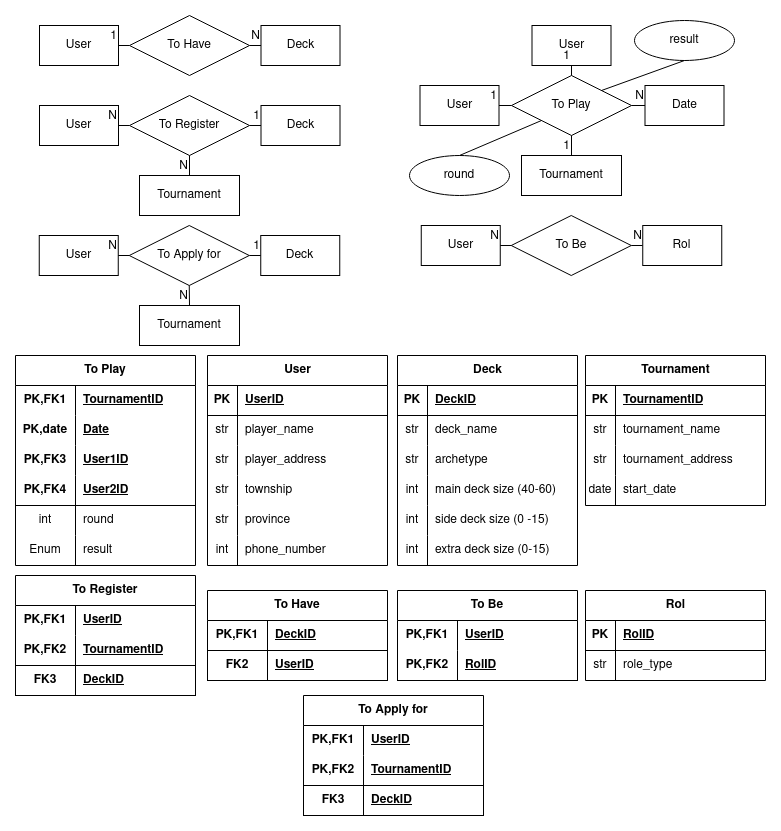
\includegraphics[width=1\textwidth]{design_with_roles.png}
  \caption{Esquema Relacional}
  \label{fig:etiqueta}
\end{figure}
\section{Valoraci\'on del dise\~no de la base de datos en cuanto a si es o no correcto:}

\end{document}
